\documentclass{extbook}[14pt]
\usepackage{multicol, enumerate, enumitem, hyperref, color, soul, setspace, parskip, fancyhdr, amssymb, amsthm, amsmath, latexsym, units, mathtools}
\everymath{\displaystyle}
\usepackage[headsep=0.5cm,headheight=0cm, left=1 in,right= 1 in,top= 1 in,bottom= 1 in]{geometry}
\usepackage{dashrule}  % Package to use the command below to create lines between items
\newcommand{\litem}[1]{\item #1

\rule{\textwidth}{0.4pt}}
\pagestyle{fancy}
\lhead{}
\chead{Answer Key for Makeup Progress Quiz 2 Version C}
\rhead{}
\lfoot{2790-1423}
\cfoot{}
\rfoot{Summer C 2021}
\begin{document}
\textbf{This key should allow you to understand why you choose the option you did (beyond just getting a question right or wrong). \href{https://xronos.clas.ufl.edu/mac1105spring2020/courseDescriptionAndMisc/Exams/LearningFromResults}{More instructions on how to use this key can be found here}.}

\textbf{If you have a suggestion to make the keys better, \href{https://forms.gle/CZkbZmPbC9XALEE88}{please fill out the short survey here}.}

\textit{Note: This key is auto-generated and may contain issues and/or errors. The keys are reviewed after each exam to ensure grading is done accurately. If there are issues (like duplicate options), they are noted in the offline gradebook. The keys are a work-in-progress to give students as many resources to improve as possible.}

\rule{\textwidth}{0.4pt}

\begin{enumerate}\litem{
Choose the graph of the equation below.
\[ f(x) = \frac{-1}{x - 2} - 1 \]The solution is the graph below, which is option D.
    \begin{center}
        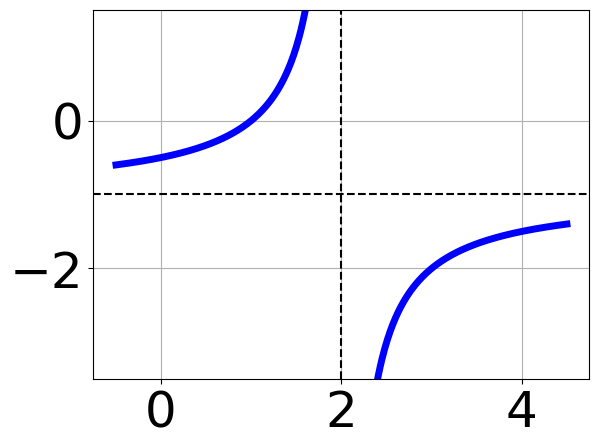
\includegraphics[width=0.3\textwidth]{../Figures/rationalEquationToGraphDC.png}
    \end{center}\begin{enumerate}[label=\Alph*.]
\begin{multicols}{2}
\item 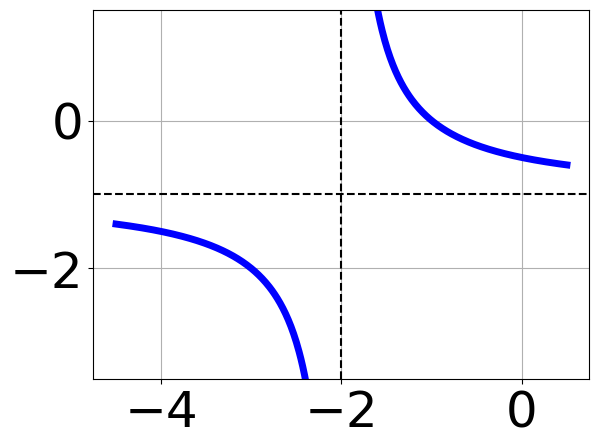
\includegraphics[width = 0.3\textwidth]{../Figures/rationalEquationToGraphAC.png}
\item 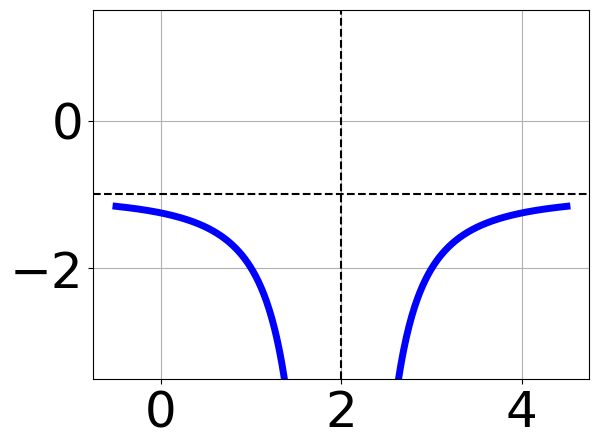
\includegraphics[width = 0.3\textwidth]{../Figures/rationalEquationToGraphBC.png}
\item 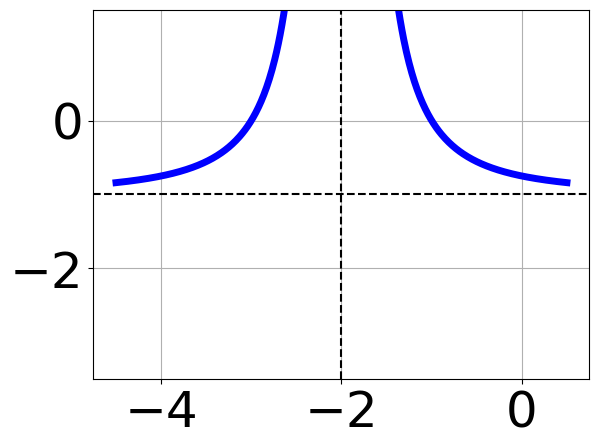
\includegraphics[width = 0.3\textwidth]{../Figures/rationalEquationToGraphCC.png}
\item 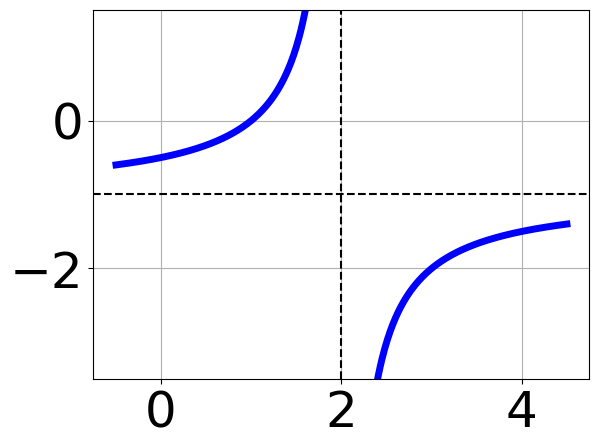
\includegraphics[width = 0.3\textwidth]{../Figures/rationalEquationToGraphDC.png}
\end{multicols}\item None of the above.\end{enumerate}
\textbf{General Comment:} Remember that the general form of a basic rational equation is $ f(x) = \frac{a}{(x-h)^n} + k$, where $a$ is the leading coefficient (and in this case, we assume is either $1$ or $-1$), $n$ is the degree (in this case, either $1$ or $2$), and $(h, k)$ is the intersection of the asymptotes.
}
\litem{
Solve the rational equation below. Then, choose the interval(s) that the solution(s) belongs to.
\[ \frac{7}{3x -8} + 8 = \frac{2}{9x -24} \]The solution is \( x = 2.403 \), which is option B.\begin{enumerate}[label=\Alph*.]
\item \( \text{All solutions lead to invalid or complex values in the equation.} \)

This corresponds to thinking $x = 2.403$ leads to dividing by zero in the original equation, which it does not.
\item \( x \in [1.4,4.4] \)

* $x = 2.403$, which is the correct option.
\item \( x_1 \in [-3.93, 0.07] \text{ and } x_2 \in [2.4,2.41] \)

$x = -2.931 \text{ and } x = 2.403$, which corresponds to getting the correct solution and believing there should be a second solution to the equation.
\item \( x_1 \in [-0.6, 5.4] \text{ and } x_2 \in [2.41,2.54] \)

$x = 2.403 \text{ and } x = 2.458$, which corresponds to getting the correct solution and believing there should be a second solution to the equation.
\item \( x \in [-3.93,0.07] \)

$x = -2.931$, which corresponds to not distributing the factor $3x -8$ correctly when trying to eliminate the fraction.
\end{enumerate}

\textbf{General Comment:} Distractors are different based on the number of solutions. Remember that after solving, we need to make sure our solution does not make the original equation divide by zero!
}
\litem{
Choose the graph of the equation below.
\[ f(x) = \frac{-1}{(x - 1)^2} + 2 \]The solution is the graph below, which is option E.
    \begin{center}
        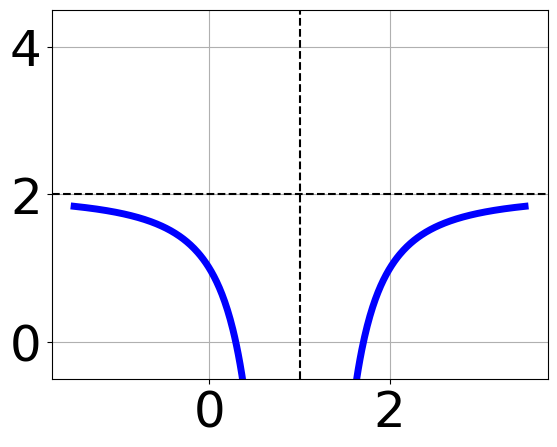
\includegraphics[width=0.3\textwidth]{../Figures/rationalEquationToGraphCopyEC.png}
    \end{center}\begin{enumerate}[label=\Alph*.]
\begin{multicols}{2}
\item 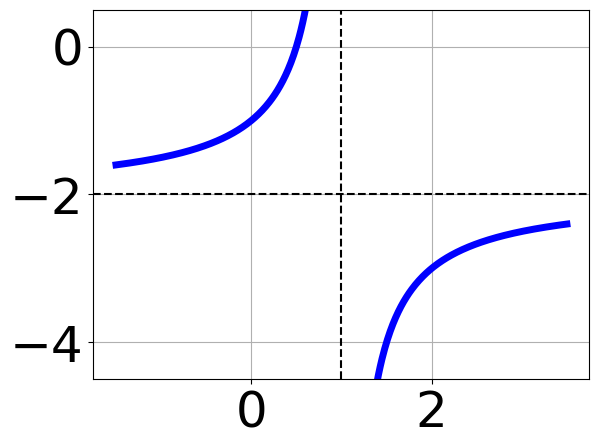
\includegraphics[width = 0.3\textwidth]{../Figures/rationalEquationToGraphCopyAC.png}
\item 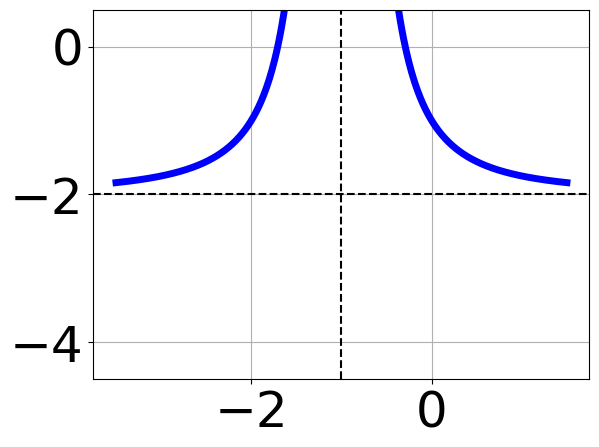
\includegraphics[width = 0.3\textwidth]{../Figures/rationalEquationToGraphCopyBC.png}
\item 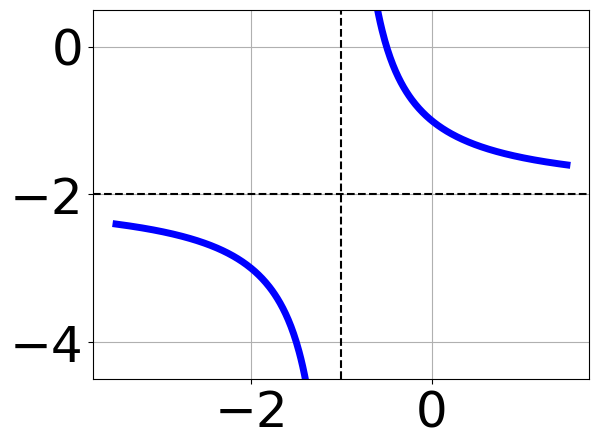
\includegraphics[width = 0.3\textwidth]{../Figures/rationalEquationToGraphCopyCC.png}
\item 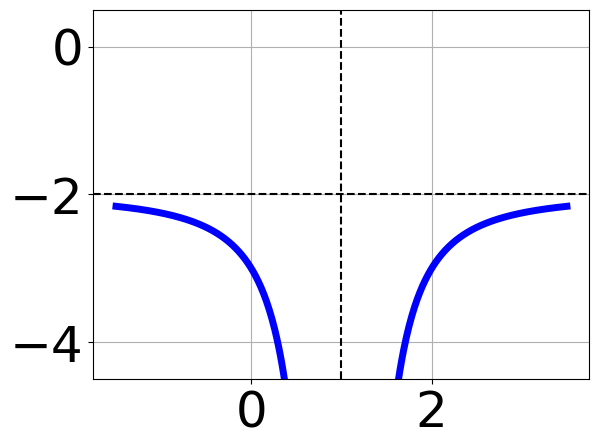
\includegraphics[width = 0.3\textwidth]{../Figures/rationalEquationToGraphCopyDC.png}
\end{multicols}\item None of the above.\end{enumerate}
\textbf{General Comment:} Remember that the general form of a basic rational equation is $ f(x) = \frac{a}{(x-h)^n} + k$, where $a$ is the leading coefficient (and in this case, we assume is either $1$ or $-1$), $n$ is the degree (in this case, either $1$ or $2$), and $(h, k)$ is the intersection of the asymptotes.
}
\litem{
Solve the rational equation below. Then, choose the interval(s) that the solution(s) belongs to.
\[ \frac{-8}{6x -3} + -5 = \frac{-7}{-36x + 18} \]The solution is \( x = 0.194 \), which is option C.\begin{enumerate}[label=\Alph*.]
\item \( x \in [-1.2,-0.4] \)

$x = -0.806$, which corresponds to not distributing the factor $6x -3$ correctly when trying to eliminate the fraction.
\item \( x_1 \in [-0.7, 1.1] \text{ and } x_2 \in [0.3,0.7] \)

$x = 0.194 \text{ and } x = 0.467$, which corresponds to getting the correct solution and believing there should be a second solution to the equation.
\item \( x \in [0.19,4.19] \)

* $x = 0.194$, which is the correct option.
\item \( \text{All solutions lead to invalid or complex values in the equation.} \)

This corresponds to thinking $x = 0.194$ leads to dividing by zero in the original equation, which it does not.
\item \( x_1 \in [-1.2, -0.4] \text{ and } x_2 \in [-0.7,0.3] \)

$x = -0.806 \text{ and } x = 0.194$, which corresponds to getting the correct solution and believing there should be a second solution to the equation.
\end{enumerate}

\textbf{General Comment:} Distractors are different based on the number of solutions. Remember that after solving, we need to make sure our solution does not make the original equation divide by zero!
}
\litem{
Determine the domain of the function below.
\[ f(x) = \frac{5}{24x^{2} +6 x -9} \]The solution is \( \text{All Real numbers except } x = -0.750 \text{ and } x = 0.500. \), which is option D.\begin{enumerate}[label=\Alph*.]
\item \( \text{All Real numbers.} \)

This corresponds to thinking the denominator has complex roots or that rational functions have a domain of all Real numbers.
\item \( \text{All Real numbers except } x = a \text{ and } x = b, \text{ where } a \in [-13, -10] \text{ and } b \in [17, 21] \)

All Real numbers except $x = -12.000$ and $x = 18.000$, which corresponds to not factoring the denominator correctly.
\item \( \text{All Real numbers except } x = a, \text{ where } a \in [-0.75, 0.25] \)

All Real numbers except $x = -0.750$, which corresponds to removing only 1 value from the denominator.
\item \( \text{All Real numbers except } x = a \text{ and } x = b, \text{ where } a \in [-0.75, 0.25] \text{ and } b \in [0.5, 3.5] \)

All Real numbers except $x = -0.750$ and $x = 0.500$, which is the correct option.
\item \( \text{All Real numbers except } x = a, \text{ where } a \in [-13, -10] \)

All Real numbers except $x = -12.000$, which corresponds to removing a distractor value from the denominator.
\end{enumerate}

\textbf{General Comment:} Recall that dividing by zero is not a real number. Therefore the domain is all real numbers \textbf{except} those that make the denominator 0.
}
\litem{
Choose the equation of the function graphed below.

\begin{center}
    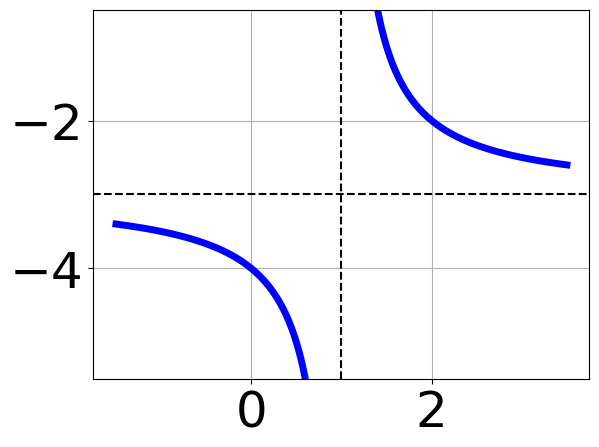
\includegraphics[width=0.5\textwidth]{../Figures/rationalGraphToEquationC.png}
\end{center}


The solution is \( \text{None of the above as it should be } f(x) = \frac{1}{x - 1} - 3 \), which is option E.\begin{enumerate}[label=\Alph*.]
\item \( f(x) = \frac{1}{x - 1} - 4 \)

The $y$-value of the equation does not match the graph.
\item \( f(x) = \frac{1}{(x - 1)^2} - 4 \)

Corresponds to thinking the graph was a shifted version of $\frac{1}{x^2}$ not noticing the $y$-value was wrong.
\item \( f(x) = \frac{-1}{x + 1} - 4 \)

Corresponds to using the general form $f(x) = \frac{a}{x+h}+k$, the opposite leading coefficient AND not noticing the $y$-value was wrong.
\item \( f(x) = \frac{-1}{(x + 1)^2} - 4 \)

Corresponds to thinking the graph was a shifted version of $\frac{1}{x^2}$, using the general form $f(x) = \frac{a}{x+h}+k$, the opposite leading coefficient, AND not noticing the $y$-value was wrong.
\item \( \text{None of the above} \)

None of the equation options were the correct equation.
\end{enumerate}

\textbf{General Comment:} Remember that the general form of a basic rational equation is $ f(x) = \frac{a}{(x-h)^n} + k$, where $a$ is the leading coefficient (and in this case, we assume is either $1$ or $-1$), $n$ is the degree (in this case, either $1$ or $2$), and $(h, k)$ is the intersection of the asymptotes.
}
\litem{
Determine the domain of the function below.
\[ f(x) = \frac{3}{20x^{2} +x -30} \]The solution is \( \text{All Real numbers except } x = -1.250 \text{ and } x = 1.200. \), which is option D.\begin{enumerate}[label=\Alph*.]
\item \( \text{All Real numbers except } x = a \text{ and } x = b, \text{ where } a \in [-21, -18] \text{ and } b \in [28, 34] \)

All Real numbers except $x = -20.000$ and $x = 30.000$, which corresponds to not factoring the denominator correctly.
\item \( \text{All Real numbers except } x = a, \text{ where } a \in [-2.25, 0.75] \)

All Real numbers except $x = -1.250$, which corresponds to removing only 1 value from the denominator.
\item \( \text{All Real numbers except } x = a, \text{ where } a \in [-21, -18] \)

All Real numbers except $x = -20.000$, which corresponds to removing a distractor value from the denominator.
\item \( \text{All Real numbers except } x = a \text{ and } x = b, \text{ where } a \in [-2.25, 0.75] \text{ and } b \in [-0.8, 3.2] \)

All Real numbers except $x = -1.250$ and $x = 1.200$, which is the correct option.
\item \( \text{All Real numbers.} \)

This corresponds to thinking the denominator has complex roots or that rational functions have a domain of all Real numbers.
\end{enumerate}

\textbf{General Comment:} Recall that dividing by zero is not a real number. Therefore the domain is all real numbers \textbf{except} those that make the denominator 0.
}
\litem{
Choose the equation of the function graphed below.

\begin{center}
    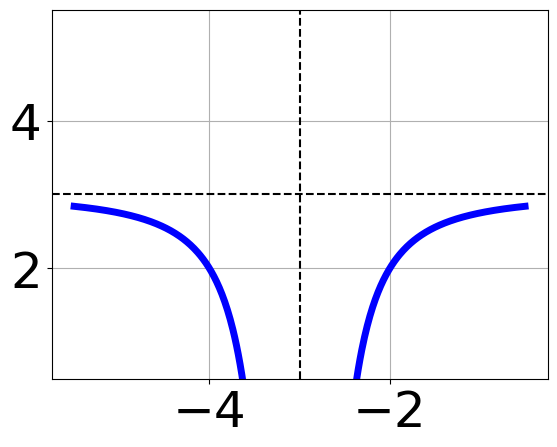
\includegraphics[width=0.5\textwidth]{../Figures/rationalGraphToEquationCopyC.png}
\end{center}


The solution is \( f(x) = \frac{-1}{(x + 3)^2} + 3 \), which is option B.\begin{enumerate}[label=\Alph*.]
\item \( f(x) = \frac{1}{x - 3} + 3 \)

Corresponds to thinking the graph was a shifted version of $\frac{1}{x}$, using the general form $f(x) = \frac{a}{(x+h)^2}+k$, and the opposite leading coefficient.
\item \( f(x) = \frac{-1}{(x + 3)^2} + 3 \)

This is the correct option.
\item \( f(x) = \frac{1}{(x - 3)^2} + 3 \)

Corresponds to using the general form $f(x) = \frac{a}{(x+h)^2}+k$ and the opposite leading coefficient.
\item \( f(x) = \frac{-1}{x + 3} + 3 \)

Corresponds to thinking the graph was a shifted version of $\frac{1}{x}$.
\item \( \text{None of the above} \)

This corresponds to believing the vertex of the graph was not correct.
\end{enumerate}

\textbf{General Comment:} Remember that the general form of a basic rational equation is $ f(x) = \frac{a}{(x-h)^n} + k$, where $a$ is the leading coefficient (and in this case, we assume is either $1$ or $-1$), $n$ is the degree (in this case, either $1$ or $2$), and $(h, k)$ is the intersection of the asymptotes.
}
\litem{
Solve the rational equation below. Then, choose the interval(s) that the solution(s) belongs to.
\[ \frac{3x}{-5x + 5} + \frac{-2x^{2}}{-35x^{2} +10 x + 25} = \frac{-2}{7x + 5} \]The solution is \( \text{All solutions are invalid or lead to complex values in the equation.} \), which is option D.\begin{enumerate}[label=\Alph*.]
\item \( x_1 \in [-0.76, -0.74] \text{ and } x_2 \in [-0.29,1.06] \)

$x = -0.759 \text{ and } x = 0.542$, which corresponds to making the discriminant from the Quadratic Formula positive to avoid complex solutions.
\item \( x \in [-0.74,-0.67] \)

$x = -0.714$, which corresponds to solving $7x + 5 = 0$ and treating it as a solution to the equation.
\item \( x \in [0.96,1] \)

$x = 1.000$, which corresponds to solving $-5x + 5 = 0$ and treating it as a solution to the equation.
\item \( \text{All solutions lead to invalid or complex values in the equation.} \)

* The equation leads to solving $23x^{2} +5 x + 10=0$, which leads to complex solutions. This is the correct option.
\item \( x_1 \in [0.96, 1] \text{ and } x_2 \in [-1.5,-0.63] \)

$x = 1.000 \text{ and } x = -0.714$, which corresponds to solving $-5x + 5 = 0$ and $7x + 5 = 0$ and treating them as solutions to the equation.
\end{enumerate}

\textbf{General Comment:} Distractors are different based on the number of solutions. Remember that after solving, we need to make sure our solution does not make the original equation divide by zero!
}
\litem{
Solve the rational equation below. Then, choose the interval(s) that the solution(s) belongs to.
\[ \frac{6x}{-6x -2} + \frac{-5x^{2}}{-18x^{2} +6 x + 4} = \frac{4}{3x -2} \]The solution is \( \text{All solutions are invalid or lead to complex values in the equation.} \), which is option E.\begin{enumerate}[label=\Alph*.]
\item \( x \in [-0.69,-0.24] \)

$x = -0.333$, which corresponds to solving $-6x -2 = 0$ and treating it as a solution to the equation.
\item \( x_1 \in [-1.03, -0.38] \text{ and } x_2 \in [0.01,0.36] \)

$x = -0.790 \text{ and } x = 0.268$, which corresponds to making the discriminant from the Quadratic Formula positive to avoid complex solutions.
\item \( x_1 \in [-0.69, -0.24] \text{ and } x_2 \in [0.59,0.96] \)

$x = -0.333 \text{ and } x = 0.667$, which corresponds to solving $-6x -2 = 0$ and $3x -2 = 0$ and treating them as solutions to the equation.
\item \( x \in [0.6,1.75] \)

$x = 0.667$, which corresponds to solving $3x -2 = 0$ and treating it as a solution to the equation.
\item \( \text{All solutions lead to invalid or complex values in the equation.} \)

* The equation leads to solving $23x^{2} +12 x + 8=0$, which leads to complex solutions. This is the correct option.
\end{enumerate}

\textbf{General Comment:} Distractors are different based on the number of solutions. Remember that after solving, we need to make sure our solution does not make the original equation divide by zero!
}
\end{enumerate}

\end{document}